\section{Implementación y programación}\label{sec:implemetacion_y_programacion}

En esta sección vamos a explicar algunos de los detalles de implementación de aquellos componentes que creemos que es
interesante que sean introducidos.

\subsection*{Componente \textit{Generator}}

\subsubsection*{PDF To Text Processor}

Como introdujimos en la sección~\ref{sec:diseno_del_sistema} Diseño del sistema, este procesador es responsable de
convertir un fichero PDF en un fragmento de texto plano.

Como puede verse en el siguiente extracto de código, el procesador \textbf{PDF To Text Processor} es simplemente un
envoltorio para \textbf{Pdf to Text}.

\lstinputlisting[language=PHP]{chapter/4/code/PdfToTextProcessor.php}

En la figura~\ref{fig:chapter_4.generator_component_pdf_to_text_processor} puede verse un esquema de este
comportamiento.

\begin{figure}[ht]
    \begin{center}
        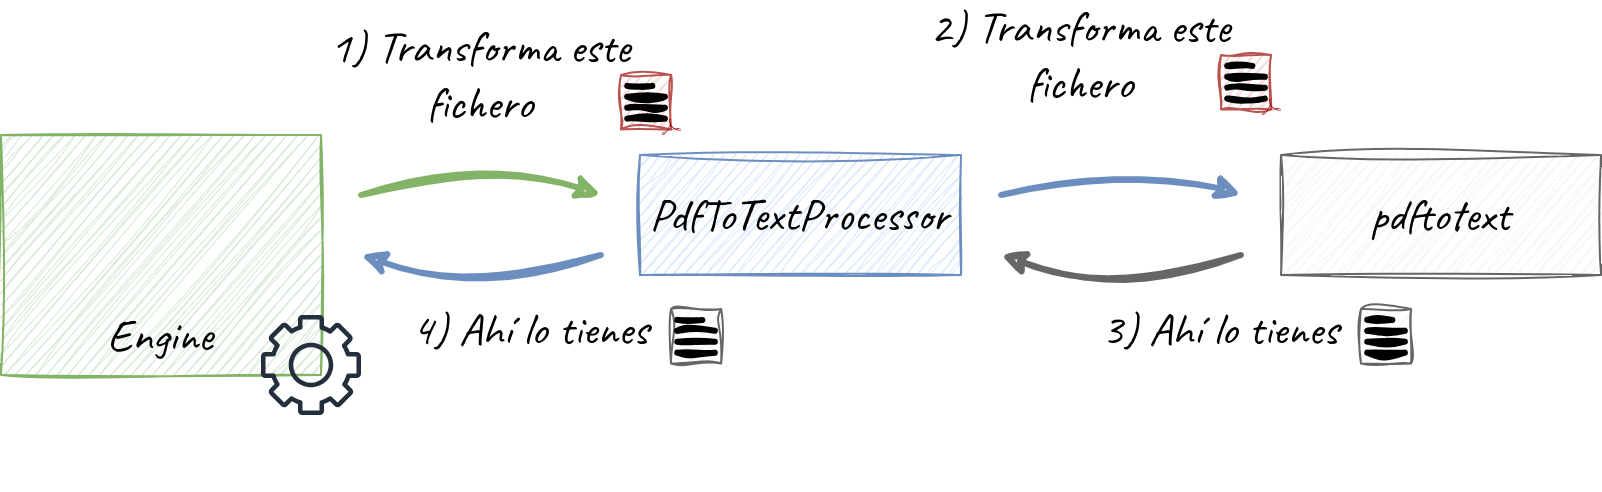
\includegraphics[width=\textwidth]{./chapter/4/images/chapter_4.generator_component_pdf_to_text_processor}
        \caption{Esquema de comunicación con pdftotext}
        \label{fig:chapter_4.generator_component_pdf_to_text_processor}
    \end{center}
\end{figure}

\subsection*{Componente \textit{Reader}}

\subsubsection*{Residential Lease Processor}

Como introdujimos en la sección~\ref{sec:diseno_del_sistema} Diseño del sistema, este procesador es responsable de
convertir transformar el texto de un contrato de arrendamiento de vivienda entre particulares en un objeto con sus
datos fundamentales.

La implementación de este procesador es muy similar a la que hemos visto en el \textbf{PDF To Text Processor}, por lo
que no vamos a incluir ni el código ni un esquema de la comunicación.

Simplemente, indicaremos que se trata de enviar peticiones sobre un documento que previamente hemos convertido en texto
plano a un sistema que lo pueda procesar, en este caso
\textbf{ChatGPT 4 Turbo}~\cite{https://platform.openai.com/docs/models/gpt-4}

Lo que si merece la pena es profundizar en los las características de las peticiones que se envían.

El primer intento de implementación se trató que el modelo respondiera con un XML. Para ello en la petición o en el
contexto se le facilitaría un XSD, que contiene los tipos de datos y sus validaciones.
Sin embargo, \textbf{ChatGPT 4} tiene limitaciones para trabajar con documentos XML, por lo que la implementación final
se realizó utilizando modelos JSON.

Como puede verse en el ejemplo de código que aparece a continuación, es vital ser muy preciso en cuanto a la
información que se le solicita y al formato en el que se espera la respuesta.
Para ello le facilitamos un ejemplo para cada tipo de dato.

\lstinputlisting[language=PHP]{chapter/4/code/ResidentialLeaseAgreementProcessor.php}

Una vez que se obtiene la respuesta en formato JSON, tan solo es necesario des-serializarlo para convertirlo en un
objeto del tipo indicado, en este caso un \textit{ResidentialLeaseAgreement} que como puede verse en el fragmento
que aparece a continuación, contiene los tipos de datos esperados para un contrato de arrendamiento de vivienda
entre particulares.

\lstinputlisting[language=PHP]{chapter/4/code/ResidentialLeaseAgreement.php}

La API de \textbf{ChatGPT 4} presenta dos problemas, es lenta y cuesta dinero.
Los tiempos de respuesta pueden variar dependiendo del tipo de documento y del estado de la api.
Los costes también pueden variar dependiendo del tipo de documento y del precio de la api en ese
momento~\cite{https://openai.com/api/pricing/}.

A continuación una tabla calculada con el promedio de 100 peticiones para este tipo de documento.

\begin{table}[h]
    \renewcommand{\arraystretch}{1.5}
    \begin{tabular}{p{0.35\textwidth} p{0.65\textwidth}}
        \hline\textbf{Total peticiones}    & 3     \\
        \hline\textbf{Tiempo total}        & 8.05  \\
        \hline\textbf{Total input tokens}  & ~6643 \\
        \hline\textbf{total output tokens} & ~159  \\
        \hline\textbf{Total price}         & ~0.07 \\
        \hline
    \end{tabular}
    \label{tab:residential_lease_processor}
\end{table}

En la fase de desarrollo de este proyecto se repiten continuamente los mismos documentos, en un ciclo de prueba y error
por lo que tanto para acelerar los tiempos de ejecución como para reducir los costes se hizo recomendable implementar
un sistema de caché.

El sistema de caché genera un token para cada petición y guarda la respuesta de dicha petición, durante un tiempo
definido.
Si se repite una misma petición recupera la respuesta de la caché, por lo que la respuesta es prácticamente
instantánea y sin ningún coste adicional.

\subsubsection*{Vehicle Sale And Purchase Processor}

Este procesador es responsable de convertir transformar el texto de un contrato de compraventa de vehículo entre
particulares en un objeto con sus datos fundamentales.

Este procesador funciona de forma tan similar al procesador anterior que no será necesario entrar en nuevos detalles
con respecto a su funcionamiento, hasta el punto de que en el momento del desarrollo fue evidente que podrían
compartir una parte muy importante del código, simplemente cambiando ligeramente las peticiones que se debían realizar.

\subsection*{Registros}

El registro de logs es una parte crucial del monitoreo y mantenimiento de cualquier aplicación.
En proyecto de este tipo, por la cantidad de pequeños componentes y por interactuar con elementos de infraestructura
externos, se hace necesario contar con un buen sistema de registro de logs.

En este proyecto, se ha implementado un sistema de registros utilizando \textbf{Monolog}, una biblioteca de registro
para PHP.

Se han configurado tres canales.

\begin{itemize}
    \item Generator: para los logs del componente generator.
    \item Reader: para los logs del componente reader.
    \item Http-Client: para el componente que realiza las peticiones HTTP.
\end{itemize}

Un canal es la forma en la que monolog, agrupa un conjunto de información para poderla filtrar y procesar adecuadamente.
Además, los logs se almacenan en dos ficheros y formatos diferentes:

\begin{itemize}
    \item \textbf{Monolog File format}, es el formato estándar de ficheros de log generados por esta biblioteca.
    \item \textbf{Logstash format}, es el estándar de la herramienta \textbf{Monolog}.
\end{itemize}

El formato \textbf{Monolog File format} está indicado para entornos de desarrollo o proyectos de pequeña envergadura.
Siempre que estos ficheros no sean demasiado grandes, se pueden trabajar a través de herramientas de línea de comandos
como \textbf{grep} o \textbf{awk}.

El formato \textbf{Logstash format} es adecuado para ser procesado por un sistema compuesto por
\textbf{Elasticsearch}, \textbf{Logstash} y \textbf{Kibana} (ELK).
Este formato está indicado en entornos de producción, donde la monitorización de los logs sea una tarea relevante.

En la figura~\ref{fig:chapter_4.logs_overview} puede verse un esquema de este comportamiento.

\begin{figure}[ht]
    \begin{center}
        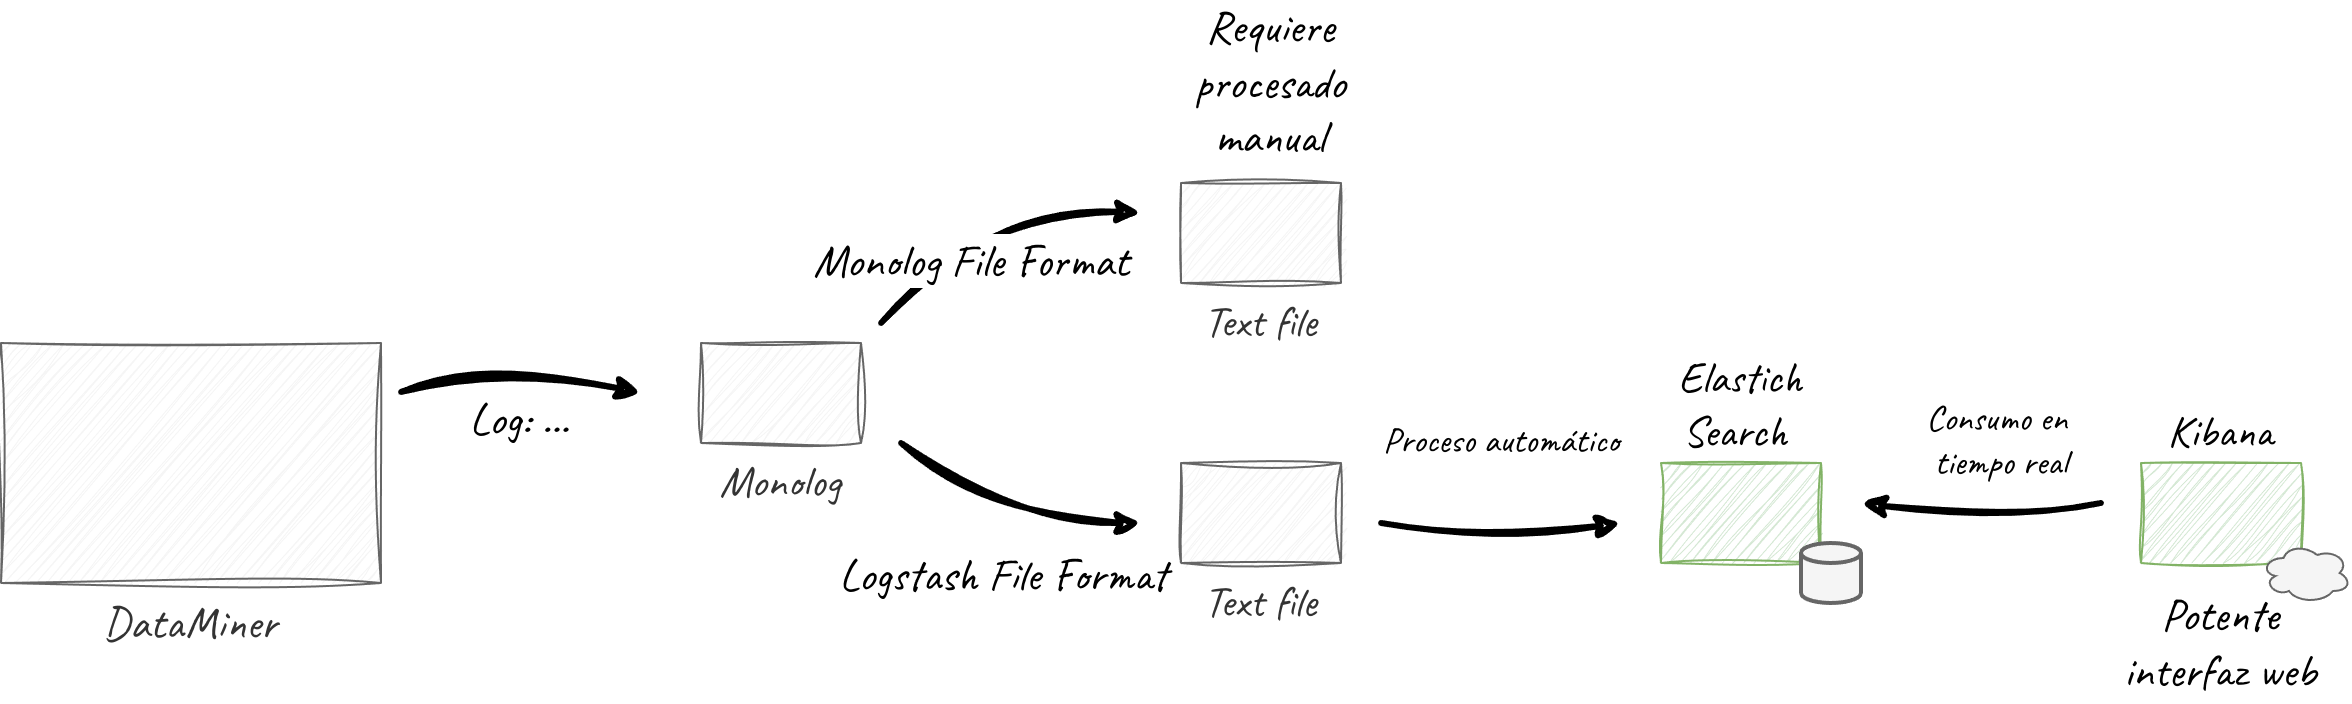
\includegraphics[width=\textwidth]{./chapter/4/images/chapter_4.logs_overview}
        \caption{Esquema del sistema de procesamiento de logs}
        \label{fig:chapter_4.logs_overview}
    \end{center}
\end{figure}